\chapter{予備評価}

\section{評価概要}

本研究では、制作した複数のグリッチライブ壁紙について、利用者がどのような表現を好むかを確認するため、予備評価を実施した。

評価実施時点では、複数のグリッチ表現を比較することで、多くの利用者から共通して高く評価される表現や、その特徴を明らかにすることを主な目的としていた。この段階では、利用者ごとの選好に応じて表現を変更するパーソナライズを主たる研究目的とはしていなかった。

評価は2026年7月に実施し、同一ゼミに所属する学生6名が参加した。参加者はいずれも比較的近い年齢層であった。本評価は、本実験に先立ってグリッチ表現に対する選好傾向を確認する探索的な予備評価として位置付ける。


\subsection{提示刺激と評価方法}

評価には、視覚的特徴の異なる8種類のグリッチライブ壁紙を使用した。各プリセットでは、配色に加え、ノイズの大きさ、RGBずれ量、パララックス量、帯状ノイズ、ちらつきの有無や強度などを変更した。

使用した8種類のプリセットと主な特徴を表\ref{tab:preliminary_presets}に示す。

\begin{table}[H]
\centering
\caption{予備評価で使用した8種類のプリセット}
\label{tab:preliminary_presets}
\begin{tabular}{lll}
\hline
番号 & プリセット名 & 主な特徴 \\
\hline
P1 & Default & 中程度のRGBずれと常時ちらつきを持つ標準的な設定 \\
P2 & Depth & パララックスを比較的強くし、端末の動きに応じてちらつく設定 \\
P3 & Vivid & 鮮やかな配色と比較的大きなRGBずれ・ノイズを持つ設定 \\
P4 & Thin & 細い帯状ノイズと小さなノイズを用い、ちらつきを抑えた設定 \\
P5 & Corrupt & 大きなノイズと強いちらつき、鮮やかな配色を持つ設定 \\
P6 & Drift & 8種類の中で最も強いパララックスを持つ設定 \\
P7 & Quiet & 小さなノイズと控えめなRGBずれを用い、ちらつきを抑えた設定 \\
P8 & Neon & RGBずれ、帯幅、色のばらつきを大きくした設定 \\
\hline
\end{tabular}
\end{table}

刺激の提示には実際のAndroid端末を使用した。評価者である著者が端末を操作し、各プリセットを順番に表示したうえで、端末を傾けることによるパララックスやグリッチ表現の変化を参加者の目前で提示した。これにより、静止画像のみでは確認できない時間的変化や端末姿勢に応じたインタラクティブな動きを含めて評価できるようにした。

8種類のプリセットは、全参加者に対して同一の順序で提示した。提示後、各プリセットについて、Google Formsを用いて「好みではない」から「好み」までの5段階で評価を求めた。

各プリセットは独立して評価する形式としたため、参加者は8種類のうち一つのみを選択するのではなく、複数のプリセットを高く評価することも、複数を低く評価することも可能であった。

なお、本評価では自由記述による回答は求めておらず、各プリセットに対する5段階評価のみを取得した。

\subsection{参加者および実施方法}

予備評価には6名が参加した。参加者はいずれも大学内の同一ゼミに所属する学生であり、年齢層も近い。

本評価は、本実験に先立ってグリッチ表現に対する選好の傾向を確認するための探索的な予備評価として実施した。そのため、参加者数および属性には偏りがあり、本評価の結果のみから一般的な選好傾向を示すことを目的とはしない。

評価にはGoogle Formsを用いた。参加者には8種類のライブ壁紙を提示し、各壁紙を確認した上で評価を行うよう求めた。

\subsection{提示刺激と評価尺度}



参加者には8種類のライブ壁紙を提示し、各壁紙について「どの程度好ましいと感じるか」を5段階で評価するよう求めた。

評価は、各刺激について独立して行う形式とした。そのため、参加者は8種類のうち一つだけを選択するのではなく、複数の壁紙を高く評価したり、反対に複数の壁紙を低く評価したりすることができる。

この方法により、各壁紙の平均的な評価傾向に加えて、同一参加者の中でどのような表現が好まれたか、また参加者間で選好がどの程度異なるかを確認することを目的とした。

\section{評価結果}

% 各プリセットについて、壁紙の例とGoogle Formsによる評価結果を示す。

\paragraph{P1：Default}

P1（Default）は、中程度のRGBずれとノイズを用い、常時ちらつきを加えた標準的な設定である。他のプリセットと比較する際の基準となる表現として構成した。P1に対する5段階評価の結果を図\ref{fig:p1_result}に示す。
\begin{figure}[H]
  \centering
  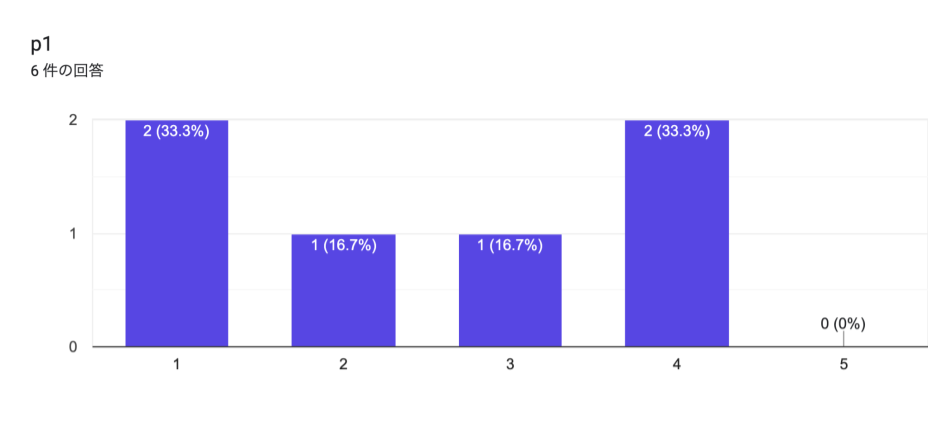
\includegraphics[width=0.75\linewidth]{figures/experiment/p1_1.png}
  \caption{P1（Default）の評価結果}
  \label{fig:p1_result}
\end{figure}

\paragraph{P2：Depth}

P2（Depth）は、端末の傾きに応じたパララックスを比較的強く設定したプリセットである。また、ちらつきを端末の動きと連動させることで、端末操作に応じた表示変化を強調している。P2に対する5段階評価の結果を図\ref{fig:p2_result}に示す。
\begin{figure}[H]
  \centering
  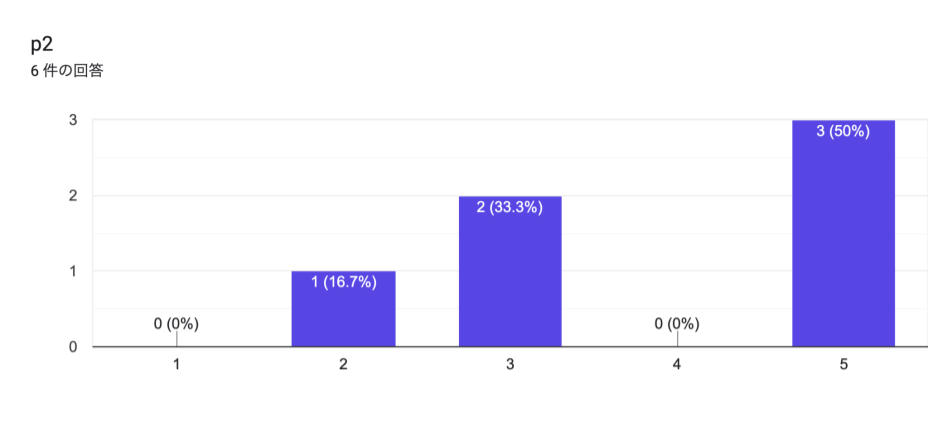
\includegraphics[width=0.75\linewidth]{figures/experiment/p2_1.png}
  \caption{P2（Depth）の評価結果}
  \label{fig:p2_result}
\end{figure}

\paragraph{P3：Vivid}

P3（Vivid）は、鮮やかな配色を用いるとともに、RGBずれおよびノイズを比較的大きく設定したプリセットである。色彩変化とグリッチの強度をともに強調した表現として構成した。P3に対する5段階評価の結果を図\ref{fig:p3_result}に示す。
\begin{figure}[H]
  \centering
  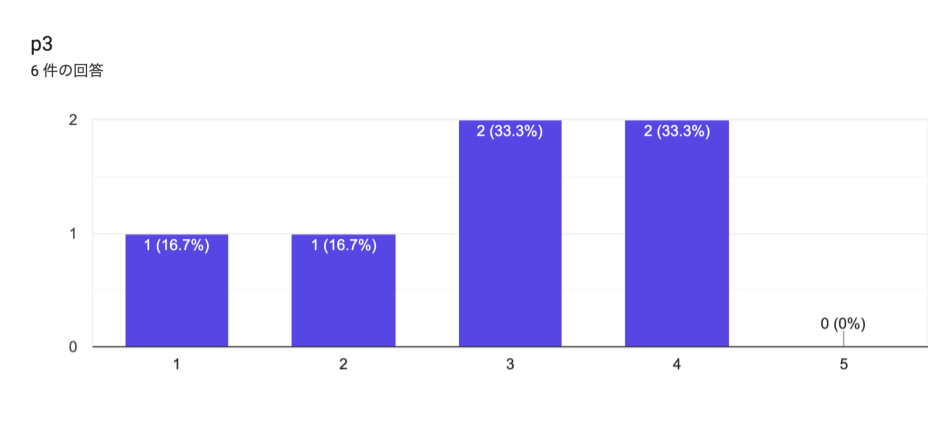
\includegraphics[width=0.75\linewidth]{figures/experiment/p3_1.png}
  \caption{P3（Vivid）の評価結果}
  \label{fig:p3_result}
\end{figure}

\paragraph{P4：Thin}

P4（Thin）は、帯状ノイズを細くし、ノイズサイズも比較的小さく設定したプリセットである。また、ちらつきを無効とすることで、他のプリセットと比較して細かく静かなグリッチ表現となるよう構成した。P4に対する5段階評価の結果を図\ref{fig:p4_result}に示す。
\begin{figure}[H]
  \centering
  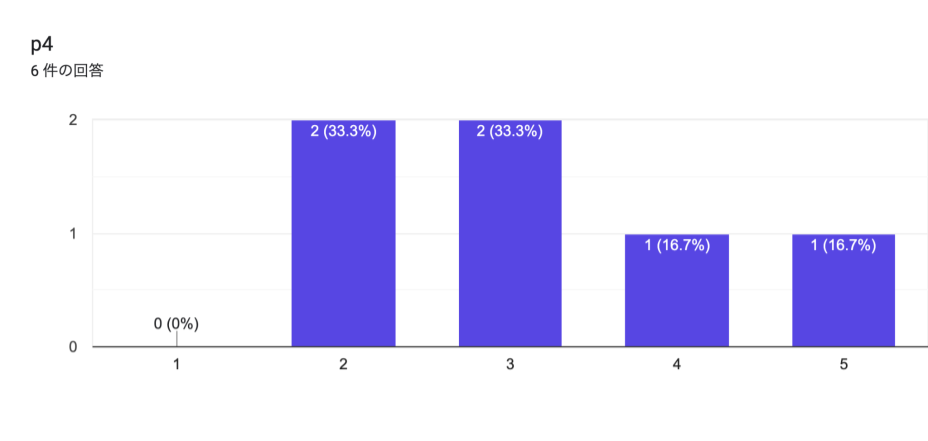
\includegraphics[width=0.75\linewidth]{figures/experiment/p4_1.png}
  \caption{P4（Thin）の評価結果}
  \label{fig:p4_result}
\end{figure}

\paragraph{P5：Corrupt}

P5（Corrupt）は、大きなノイズと強いちらつきを用い、画面の破損感を強調したプリセットである。また、鮮やかな配色を組み合わせることで、視覚的な変化量の大きい表現として構成した。P5に対する5段階評価の結果を図\ref{fig:p5_result}に示す。
\begin{figure}[H]
  \centering
  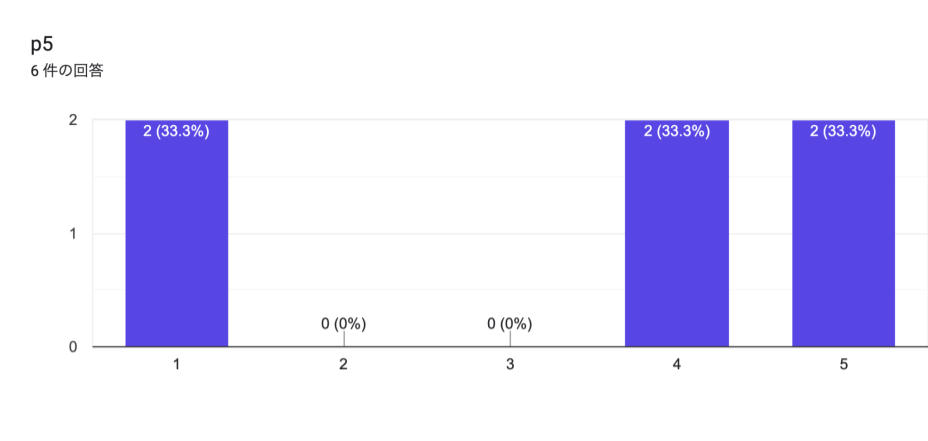
\includegraphics[width=0.75\linewidth]{figures/experiment/p5_1.png}
  \caption{P5（Corrupt）の評価結果}
  \label{fig:p5_result}
\end{figure}


\paragraph{P6：Drift}

P6（Drift）は、8種類のプリセットの中で最もパララックスを強く設定したものである。端末を傾けた際のレイヤ間の移動量の差を大きくすることで、グリッチ要素の移動と擬似的な奥行き感を強調した。P6に対する5段階評価の結果を図\ref{fig:p6_result}に示す。
\begin{figure}[H]
  \centering
  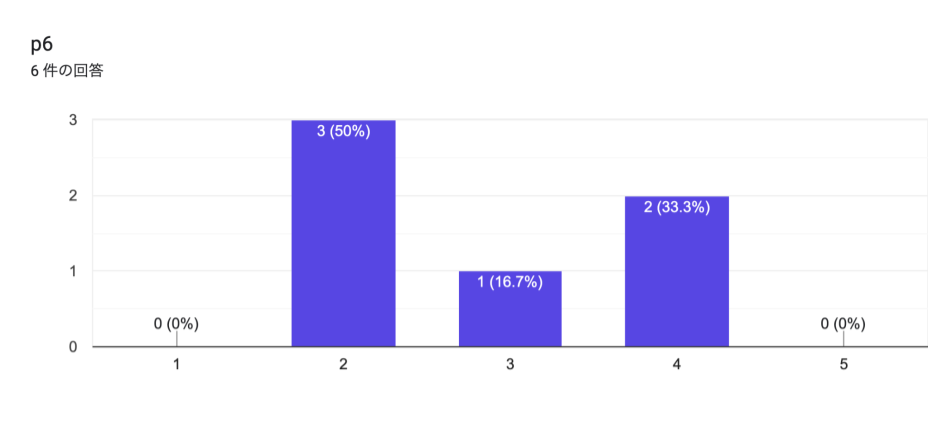
\includegraphics[width=0.75\linewidth]{figures/experiment/p6_1.png}
  \caption{P6（Drift）の評価結果}
  \label{fig:p6_result}
\end{figure}

\paragraph{P7：Quiet}

P7（Quiet）は、小さなノイズと控えめなRGBずれを用い、ちらつきを無効としたプリセットである。グリッチ表現の視覚的な刺激を比較的抑えた構成としている。P7に対する5段階評価の結果を図\ref{fig:p7_result}に示す。
\begin{figure}[H]
  \centering
  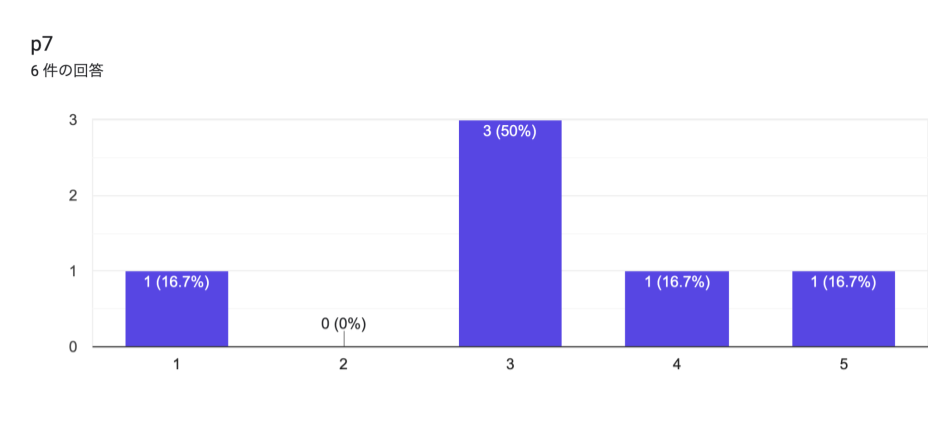
\includegraphics[width=0.75\linewidth]{figures/experiment/p7_1.png}
  \caption{P7（Quiet）の評価結果}
  \label{fig:p7_result}
\end{figure}

\paragraph{P8：Neon}

P8（Neon）は、RGBずれ、帯状ノイズの幅、色のばらつきを8種類の中で大きく設定したプリセットである。色成分の分離と広い帯状の変化を組み合わせ、色彩的なグリッチ表現を強調した。P8に対する5段階評価の結果を図\ref{fig:p8_result}に示す。
\begin{figure}[H]
  \centering
  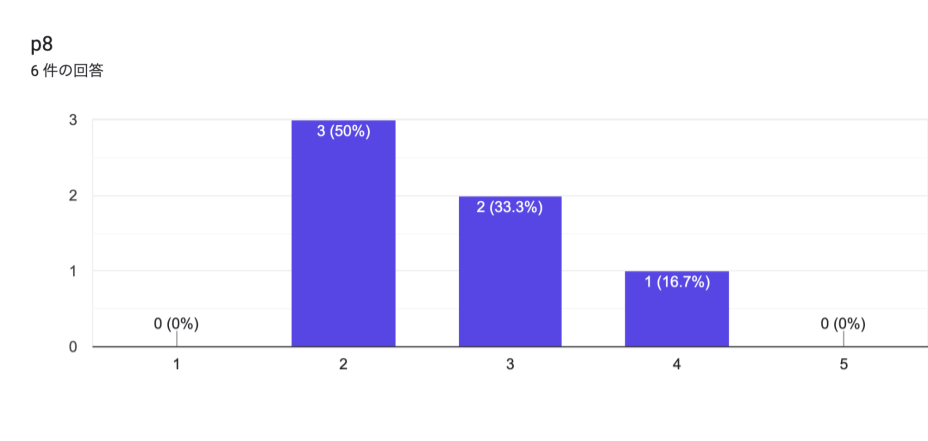
\includegraphics[width=0.75\linewidth]{figures/experiment/p8_1.png}
  \caption{P8（Neon）の評価結果}
  \label{fig:p8_result}
\end{figure}

\subsection{評価結果のまとめ}

8種類のライブ壁紙に対する評価を比較すると、特定のプリセットがすべての参加者から一様に支持される傾向は見られず、各壁紙に対する評価には参加者間でばらつきが確認された。特に、グリッチの強度、色彩、RGBずれ、視差効果などの異なる特徴を持つ壁紙に対して、参加者ごとの評価傾向は一様ではなかった。

この結果から、ライブ壁紙におけるグリッチ表現には単一の最適な設定を定めることが難しく、ユーザによって好まれる表現が異なる可能性が示唆された。本予備評価は、本研究において表現のパーソナライズへ着目する契機となった。そこで以降のシステムでは、あらかじめ定めたプリセットのみを提示するのではなく、ユーザ自身がグリッチの種類や強度、色彩等を調整できる構成へと設計方針を変更した。

\section{考察と今後の方針}

本評価では、当初、8種類のグリッチ表現を比較することで、多くの利用者から共通して高く評価される表現を明らかにすることを想定していた。

しかし、評価結果では、特定の一種類のみがすべての参加者から一貫して高く評価される傾向は確認できなかった。参加者によって高く評価する壁紙が異なり、同一のグリッチ表現に対する評価にも差がみられた。

この結果から、本研究で扱うグリッチ表現について、単一の表現を最適なものとして決定するだけでは、利用者ごとの選好の違いを十分に扱えない可能性があると考えた。そこで、予備評価以降は、一つの最適なグリッチ表現を探索する方向から、利用者が自身の選好に応じて異なる表現を選択できる構成を検討する方向へ研究方針を変更した。

ただし、本評価の参加者は6名と少なく、同一ゼミに所属する近い年齢層の学生に限定されている。また、評価項目も各壁紙に対する好ましさの5段階評価のみであり、参加者がどの視覚的要素を理由として評価したのかまでは明らかにできていない。

したがって、本評価の結果は一般的な利用者全体の選好を示すものではなく、今後の評価方法およびシステム設計を検討するための予備的な結果として位置付ける。